\documentclass{article}
% translate with >> pdflatex -shell-escape <file>

% This file is an extract of the PGFPLOTS manual, copyright by Christian Feuersaenger.
% 
% Feel free to use it as long as you cite the pgfplots manual properly.
%
% See
%   http://pgfplots.sourceforge.net/pgfplots.pdf
% for the complete manual.
%
% Any required input files (for <plot table> or <plot file> or the table package) can be downloaded
% at
% http://www.ctan.org/tex-archive/graphics/pgf/contrib/pgfplots/doc/latex/
% and
% http://www.ctan.org/tex-archive/graphics/pgf/contrib/pgfplots/doc/latex/plotdata/

\usepackage{pgfplots}
\pgfplotsset{compat=newest}

\pagestyle{empty}

\begin{document}
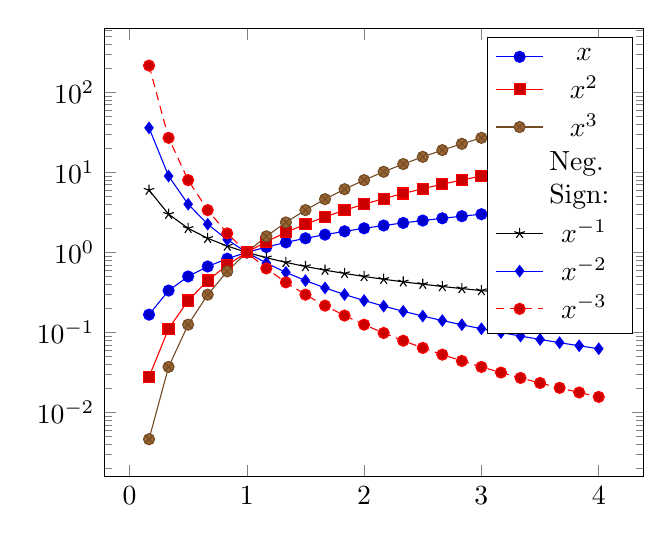
\begin{tikzpicture}
\begin{semilogyaxis}[
	domain=0:4,
	legend entries={%
	  $x$,$x^2$,$x^3$,%
	  {[text width=25pt,text depth=]Neg. Sign:},%
	  $x^{-1}$,$x^{-2}$,$x^{-3}$},
	% same effect:
	% legend style={
	% 	nodes={text width=25pt,text depth=}}
]
	\addplot {x}; 
	\addplot {x^2};
	\addplot {x^3};
	\addlegendimage{empty legend}
	\addplot {x^(-1)};
	\addplot {x^(-2)};
	\addplot {x^(-3)}; 
\end{semilogyaxis}
\end{tikzpicture}
\end{document}
